\section{Discussion}

On a présenté les fonctions noyau et l'analyse par composantes principales avec noyaux. L'idée de la méthode est la suivante : au lieu de faire une décomposition par valeurs et vecteurs propres de la matrice variance covariance des données $\textbf{x}$, on doit faire une décomposition par valeurs et vecteurs propres de la matrice des noyaux. Or, on effectue un ACP sur une projection des données vers un espace où il est possible d'expliquer la variation par les données de manière non-linéaire. On a présenté le truc du noyau : il n'est pas nécessaire de calculer directement les données projetées pour effectuer une ACP car on peut substituer le produit scalaire entre les données par une fonction noyau. \\

Ces méthodes ont notamment été utilisés dans la détection d'attributs dans la reconnaissance faciale, voir \cite{kim2002face}. 

\subsection{Avantages}

Comme mentionné précédemment, l'ACP avec noyau permet de faire une ACP sur une transformation non-linéaire des données. Les méthodes à noyaux ont eus beaucoup de succès dans les tâches de classification et de régression car il est possible de trouver une espace où un hyperplan séparateur pourrait parfaitement séparer les données. Dans le contexte de l'ACP, cette méthode peut permettre de découvrir des relations non-linéaire et bien représenter la variabilité des données dans un nombre plus retreint de composantes principales et pourrait aider à mieux interpréter les composantes. \\

Par exemple, dans le jeu de données jouet, il n'était pas possible de réduire la dimension des données car les relations étaient circulaires, on devait garder toute la dimension des données pour comprendre la distribution des classes. Avec un noyau Gaussien, il était possible de représenter et interpréter les données avec une seule composante.

\subsection{Désavantages}

Les fonctions à noyau sont très flexibles, mais on doit souvent ajuster des hyperparamètres pour avoir une représentation des données qui est utile pour l'interprétation. Dans notre application, il était simple de distinguer les bonnes projections des mauvaises, car les étiquettes de classe étaient disponibles. Dans le contexte de découverte d'information.\\

Une propriété intéressante de l'ACP est qu'on peut reconstruire les données en gardant toutes les composantes. Dans notre cas, on ne peut pas les reconstruire car ces données se trouvent dans un espace $\mathcal{F}$ qui n'est pas toujours connu. Avec l'ACP appliqué en vision, il est possible de visualiser l'information conservé. Par exemple, on recréer les images originales avec l'ACP mais en ne conservant que dix composantes principales. On obtient 

\begin{figure}[H]
	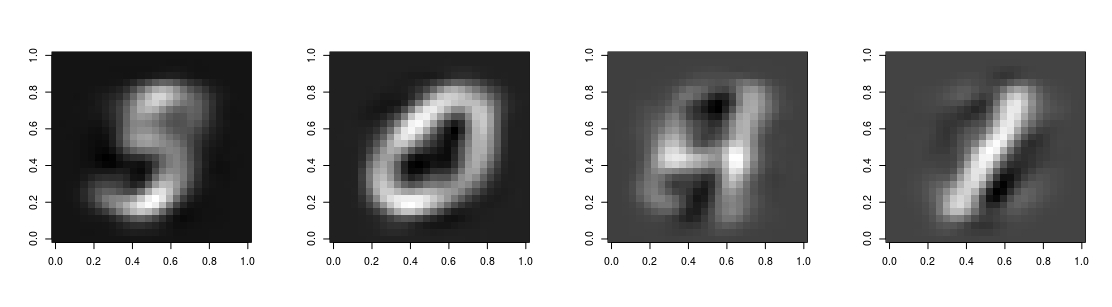
\includegraphics[width=\textwidth]{reconstruction}
	\caption{Données reconstruites avec 10 composantes principales}
	\label{fig:reconstruit}
\end{figure}

On remarque qu'on humain peut distinguer les chiffres dans la figure \ref{fig:reconstruit}. Par contre, on ne peut pas faire cette même projection avec les données dans l'espace $\mathcal{F}$ car elles ne sont jamais calculées. Ainsi, la meilleure manière d'évaluer la qualité de l'ACP avec noyau est d'étudier la proportion de l'information des noyaux qui est expliqué par les premières composantes principales. 
